%Autores: Prof. Me. Phyllipe Lima
%         Daylon Ramos da Silva
%Contato: phyllipe_slf@yahoo.com.br
%         biblioteca.pesquisa@inatel.br
%Modelo para escrita de artigos científicos para o INCITEL - CONGRESSO DE INICIAÇÃO CIENTÍFICA DO INATEL 

%Se você é novo no latex, um bom lugar para começar é
%https://pt.overleaf.com/learn
\documentclass[10pt,conference]{inatel} 
%Use esse arquivo para incluir novos pacotes

\usepackage[%usado para determinar medidas
top=1.78cm,
bottom=1.78cm,
left=1.65cm,
right=1.65cm,
headsep=0cm,
%showframe
]{geometry}
%\usepackage[justification=centering]{caption}
\usepackage{times}
\usepackage{enumitem}%redefinir espacos itemize
\usepackage{graphicx}
\usepackage{url,hyperref}
\usepackage[utf8]{inputenc}
\usepackage{float}%mais controle para manipular figuras
\usepackage{caption}%manipular legenda da figura e tabela
\usepackage{mathtools}%equacoes
\usepackage[hang,flushmargin]{footmisc} 
\usepackage{xcolor}
\usepackage{wrapfig} %usado para envolver figura com texto
%\usepackage[portuguese]{babel}
\usepackage{fancyhdr}%criacao do cabecalho
\usepackage{etoolbox}
\usepackage[export]{adjustbox}%mais controle para ajustar tamanho da tabela
\usepackage{comment}%ambiente para comentario
\usepackage{relsize} %usado por comandos \mathlarger

%Referencia bibliografica
\usepackage[
    style=numeric,
    sorting=none,
    maxbibnames=10]{biblatex}
\addbibresource{referencia.bib}

%Idioma. Use "english" para trabalhos em inglês
\usepackage[english]{babel}

%Ajustes na legenda da figura. Incluindo espacamento apos a legenda
\captionsetup[figure]{labelformat={default},labelsep=period,font=footnotesize, name=\footnotesize{Fig.},justification=centering,singlelinecheck=false,belowskip=-0.9\normalbaselineskip}
%\pagenumbering{gobble}

%Ajustes na legenda da tabela. 
\captionsetup[table]{labelformat={default},labelsep=newline,font={sc,footnotesize},justification=centering,singlelinecheck=false}

%\renewcommand{\headrulewidth}{0pt}

\makeatletter
\newcommand{\linebreakand}{%
  \baselineskip 
  \end{@IEEEauthorhalign}
  \hfill\mbox{}\par
  \mbox{}\hfill\begin{@IEEEauthorhalign}
}
\makeatother


%%%%%%%%%%%%%%%%%%%%%%%%%%%%%%%%%%%%%%%%%%%%%%%%%%%%%%%%%%%%%%%%%%%%%%%%%
%    Configuracaoes de Idioma
%    Considerando babel = brazil
%%%%%%%%%%%%%%%%%%%%%%%%%%%%%%%%%%%%%%%%%%%%%%%%%%%%%%%%%%%%%%%%%%%%%%%%% 

\addto\captionsbrazil{
  \renewcommand{\abstractname}{Abstract}
  \renewcommand{\tablename}{TABELA}
}

%considerando babel = english
\addto\captionsenglish{
  \renewcommand{\tablename}{TABLE}
}



\begin{document}


  \title{Instruções Para os Autores}
  \author
  {
    \IEEEauthorblockN{Carlos Alberto Ynoguti, Rosanna Mara Rocha Silveira, Phyllipe Lima\\}
    \IEEEauthorblockA{Instituto Nacional de Telecomunicações - Inatel\\
                  ynoguti@inatel.br, rosannas@inatel.br, phyllipe@inatel.br}
  }

\maketitle

\begin{abstract}
   This document contains information on the preparation of the final
   version of a paper accepted for publication in the Scientific Congress of Inatel, INCITEL. Please carefully follow the instructions provided to ensure legibility and uniformity of accepted papers. 
  \end{abstract}

  \begin{IEEEkeywords}
    About four keywords or phrases in alphabetical order, separated by commas.
  \end{IEEEkeywords}

  \begin{resumo}
    Este documento contém informações para a preparação da versão final de um artigo aceito para publicação no Congresso de Iniciação Científica do Inatel, INCITEL. Por favor siga cuidadosamente as instruções para garantir a legibilidade e uniformidade dos artigos aceitos.
  \end{resumo}
  
  \begin{palavraschave}
    
    Aproximadamente quatro palavras chave ou frases em ordem alfabética, separadas por vírgulas.
  \end{palavraschave}
\section{Main Ideas}
Image classification challenge has been one of the most-discussed problems in the past decades. However, better and better network structures have been found, whose accuracy on natural image classification has risen to an extent of general satisfactory among almost all datasets, except for medical segmentation tasks. Medical image segmentation is still challenging because of its importance as a nature and its commitment for finding tiny structures which could affect diagnosis results.\\

Some Challenges have been asking for better methods for medical image segmentation, like ISBI. During the search for domain-specific networks, we noted that there are three networks in a series all belonging to the U-Net school, which, seen in a row, can uncover the progress the field very well. These methods are: U-Net, UNet++ and UNet+++.\\

We did experiments on these methods with the provided ISBI dataset, compared the procedure of leveraging all these methods and listed the performances of all. Although all three methods are all implemented on different machines with different calculation capacities, the experiments could still uncover some interesting traits among all these methods. The results of all methods show that UNet+++ performs best, with an accuracy of 0.923, with U-Net following it at 0.919, and UNet++ ranking the worst at 0.917. We also did more comparison in the final section.

\section{Instruções Gerais}
Quando escrever o seu artigo, por favor atente às seguintes instruções:

\subsection{Tamanho e formato do papel}
Os trabalhos serão impressos em papel tamanho carta (letter), exatamente como você os submeter. Desta forma, a organização e o esmero são de extrema importância Por favor, faça uma revisão cuidadosa dos erros gramaticais e de digitação antes da submissão. Há um limite máximo de 6 e mínimo de 4 páginas para o artigo. Contamos com o bom senso dos autores neste caso.

Os artigos devem ser preparados em coluna dupla. Defina as margens superior e inferior em 1,78 cm, as margens esquerda e direita em 1,65 cm. As colunas devem ter largura de 8,89 cm e o espaço entre elas devem ser de 0,51 cm. Use espaçamento simples entre as linhas.

\subsection{Resumo e abstract}
Os artigos escritos em língua portuguesa devem ter também o resumo e as palavras-chave traduzidos para a língua inglesa, como neste exemplo. Garanta que tanto o \textit{abstract} quanto o resumo tenham no máximo 150 palavras.

\subsection{Seções e subseções}
As seções devem ser numeradas com algarismos romanos e ter o título centralizado. Já as subseções devem ser numeradas com letras maiúsculas e ter o título justificado, caso haja sequência de subtítulos as letras devem ser minúsculas e justificadas. 

\subsubsection{Sub-subseção}

Exemplo de uma sub-subseção.

\subsection{Figuras e Tabelas}

Figuras e Tabelas devem ser incluídas como parte do texto sempre que possível, caso contrário, agrupe-as ao final do texto. As Figuras não devem ter elementos coloridos e seus rótulos devem ser posicionados depois das mesmas, com alinhamento centralizado. A sua numeração deve ser feita com algarismos arábicos. Para as Tabelas, o procedimento é diferente: seus rótulos devem ser posicionados antes das mesmas, centralizados, e a numeração deve ser feita com algarismos romanos. As figuras devem ser referenciadas no texto, da seguinte forma: A Figura \ref{fig:incitel} apresenta o logo do INCITEL.

\begin{figure}[h]
    \centering
    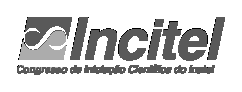
\includegraphics{figuras/logo_incitel.eps}
    \caption{Uma figura. O título deve ser colocado abaixo da mesma.}
    \label{fig:incitel}
\end{figure}

\subsection{Equações}
A numeração das equações deve ser entre parênteses e alinhada à direita, como no exemplo abaixo:

\begin{equation}
\label{eq:mgf}
\phi_X(s)=E[e^{sx}]
\end{equation}

%Consulte a página 
Para mais símbolos matemáticos, consulte o LaTeX wiki \cite{latexMath}

\subsection{Fontes}

Use fonte do tipo Times New Roman ou similar. Os tamanhos a serem usados são mostrados na Tabela \ref{tab:tabela1}

\begin{table}[h]
\centering
\caption{Tamanhos e Tipos de Letras}
\label{tab:tabela1}
\begin{adjustbox}{max width=\textwidth}
\begin{tabular}{|c|c|c|}
\hline
TEXTO & TAMANHO & ESTILO \\ \hline\hline
Título                      & 24pt                         & Negrito                     \\
Nome do autor               & 11pt                         & Normal                      \\
Afiliação                   & 10pt                         & Normal                      \\
Texto principal             & 10pt                         & Normal                      \\
Título das seções           & 10pt                         & Caixa Alta                  \\
Título das subseções        & 10pt                         & Itálico                     \\
Título do resumo/abstract   & 9pt                          & Negrito,Itálico             \\
Resumo/Abstract             & 9pt                          & Negrito                     \\
Título das figuras          & 8pt                          & Normal                      \\
Título das tabelas          & 8pt                          & Caixa Alta                  \\
Texto das tabelas           & 8pt                          & Normal                      \\
Referências                 & 8pt                          & Normal                      \\ \hline
\end{tabular}
\end{adjustbox}
\end{table}


%Se desejar, consulte a página \url{https://www.tablesgenerator.com} para criar a estrutura da sua tabela em latex. Esta página fornece uma interface gráfica que facilita a geração de tabelas em latex. Depois de gerado o código fonte pela página, insira este código no seu texto e faça os ajustes necessários.

\subsection{Referências bibliográficas}

Liste as referências em ordem numérica ao final do artigo. Ao final deste texto tem-se vários exemplos de como listá-las, dependendo do tipo. Denote as citações dentro do texto através de colchetes (por exemplo \cite{LIMA2018}). Ao referenciar mais de um trabalho, use o mesmo par de colchetes, como exemplo: \cite{LIMA2018, schell2014, Lima2017}. 

Segue um exemplo para citações textuais: ``De acordo com \textcite{LIMA2018}'' 


\subsection{Outras questões}
Não use notas de rodapé a menos que sejam estritamente necessárias; neste caso, procure não agrupá-las. 
\section{Methods}
\subsection{U-Net}
\subsubsection{Motivation}
Here we explain why we choose U-Net as our first and baseline method to experiment with. Published in \cite{unet}, it has been cited over 10000 times and widely used as a benchmark in medical image segementation. Based on U-Net, many vairations are designed to pursue better performance, as we will see in later parts. Nevertheless, U-Net itself was a big breakthrough at its publish time, and it is very beneficial to study with its netwrok structure.

\subsubsection{Detailed Description}
Image segementation has long been a major task in computer vision, where the input is an image and the expected output is the mask of image\textemdash where all pixels belonging to the same object are labeled out (See Figure~\ref{fig:sege}). 
\begin{figure}[!htpb]
    \centering
    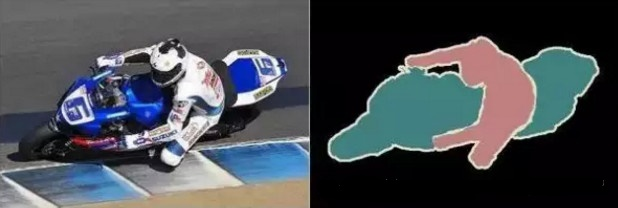
\includegraphics[scale=0.3]{figuras/segementation.jpg}
    \caption{An illustration of the goal of iamge segementation.}
    \label{fig:sege}
\end{figure}

The first try to combine deep learning methods with this task is Fully Convolutional Networks by \cite{FCN}, which became a milestone. We know that in traditional CNN, the feature dimension is decreased by convolution and pooling operations, and the reception region change from local to global gradually as the image propagate through the network. This makes it difficult to do segementation, as we have to restore the size of image. FCN uses reversed convolution and upsampling operation to restore image size, and conduct pixel-level classification.
\begin{figure}[!htpb]
    \centering
    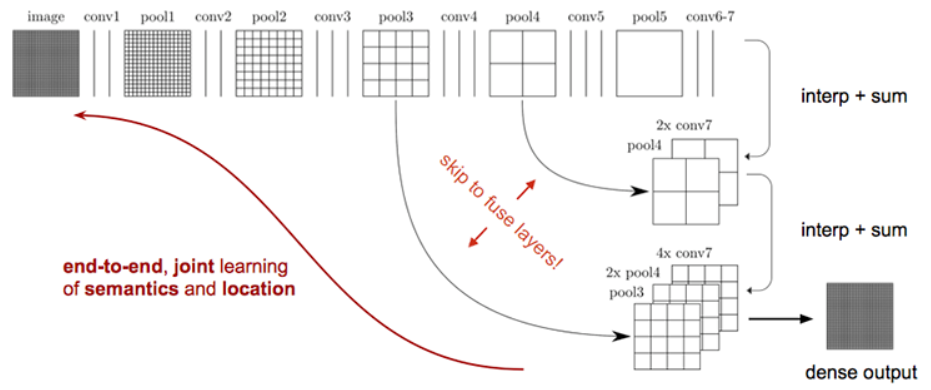
\includegraphics[scale=0.3]{figuras/FCN.PNG}
    \caption{Structure of Fully Convolutional Network, where it fuses pool4, pool3 and feature map to concate features.}
    \label{fig:fcn}
\end{figure}

However, FCN is not good at image details (see Figure~\ref{fig:fcnd}). The result is often blurred and smooth, thus not suitable for medical image segementation, where we especailly care about edges and details in the image, in case the doctors make wrong diagnosis. So there came U-Net, which imporve based on FCN. 

\begin{figure}[!htpb]
    \centering
    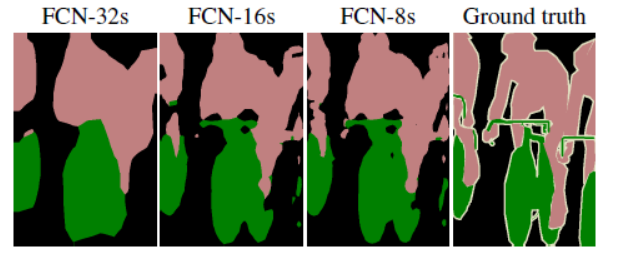
\includegraphics[scale=0.5]{figuras/FCNdetail.PNG}
    \caption{Some results of FCN compared with the ground truth. Details of the cycling man isn't very good.}
    \label{fig:fcnd}
\end{figure}

Figure~\ref{fig:unets} shows the structure of U-Net. It uses many feature channels to allow features containing more information on the texture of original image to propagate between high-resolution layers. And it is specaily designed for medical tasks, where it is very difficult to separate the connected same-category cells. The authors proposed weighted loss function, where it gives the ground truth of connected cells more consideration. U-Net can perform well on small datasets like ISBI challenge, and does not require demanding GPU memory. Of course, data augmentation needs to be done before training.

\begin{figure}[!htpb]
    \centering
    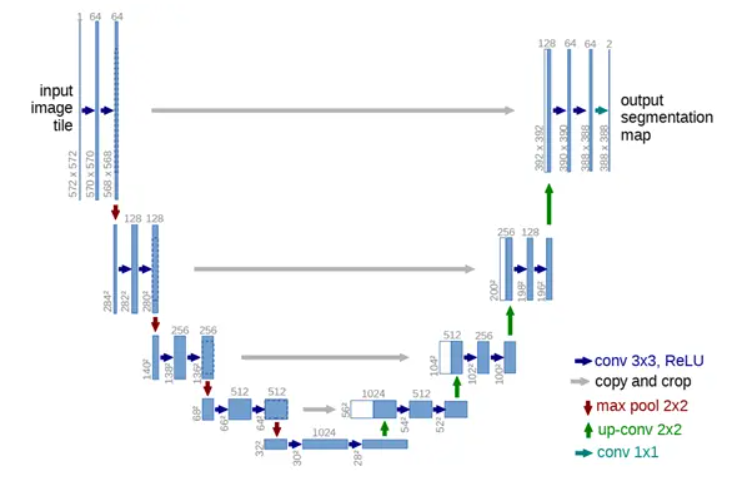
\includegraphics[scale=0.4]{figuras/unet.PNG}
    \caption{Sructure of U-Net. It looks like the character `U'. }
    \label{fig:unets}
\end{figure}
%\section{Methods}
\subsection{UNet++}
\subsubsection{Motivation}
It's clear that methods before UNet++\cite{unet_pp} can solve general image segmentation problem with decent accuracy, especially when segmenting natural images. However, medical image segmentation require more accuracy in the detail of the segmentation, for example, tumors with ragged edges and more blood vessels on the edge are more likely to be malignant. This puts a higher target for neural networks dedicated to solving medical image segmentation problem, calling for higher-accuracy methods. Also, it's hard for U-Net users to prune U-Net architecture to gain optimal inference time.\\
As a result, two propositions have been made:
\begin{itemize}
    \item Better networks are needed to solve medical image segmentation problems;
    \item Networks need to be more friendly to production situations where recognition speed is vital.
\end{itemize}
In order to meet these requirements, UNet++ was designed above U-Net\cite{unet} with skip connections replaced with dense convolution blocks. We will discuss detailed designs in the next section.

\subsubsection{Detailed Description}
The biggest modification from U-Net into UNet++ was its skip connections. Where were direct skip connections in U-Net was replaced with an array of dense convolutional layers, reforming the network shape as shown in Figure.\ref{fig:unetppStructure}.

\begin{figure}[!htpb]
\centering
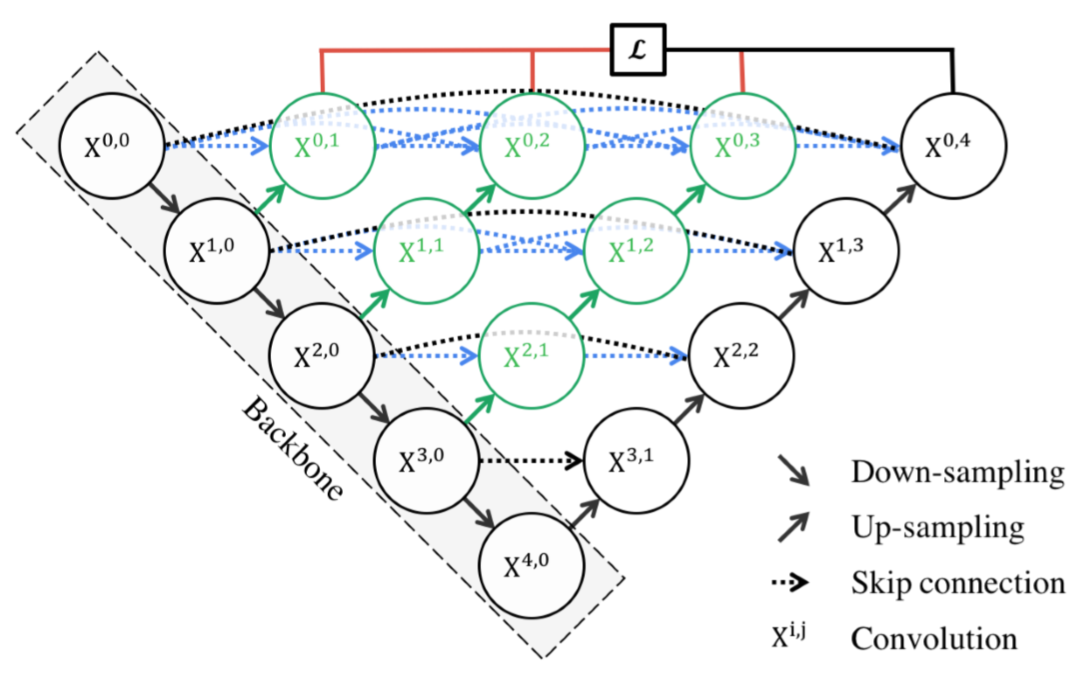
\includegraphics[scale=0.3]{figuras/unetppStructure.png}
\caption{Structure of Unet++, where black nodes represent basic U-Net, green nodes are dense convolution layers, blue and green arrows are dense connections and up-sampling, and red connections represent deep supervision.}
\label{fig:unetppStructure}
\end{figure}

The basic idea of UNet++ was that, with more dense convolution layers in between, the encoder activation domain would become closer to the decoder network activation domain, thus making finding exact segmentation a easier job. From another perspective, the network structure of UNet++ can be separated into several independent networks, as shown in Figure\ref{fig:unetppPrune}, there was 4 of them, each having more layers than the last, inheriting the last one's encoder feature map, and adding another layer beyond that. Applying loss at all 4 output positions for the full-fledged network leverages the popular deep supervision method, not only helping the network to converge better, but also enabling users to prune the network during inference time as users can only use the first several layers of output to determine the result. Consequently, UNet++ with its special dense convolution connections could deal with the two requirements that we mentioned at the same time, thus being more strong and efficiency-aware than bare U-Net.

\begin{figure}[!htpb]
\centering
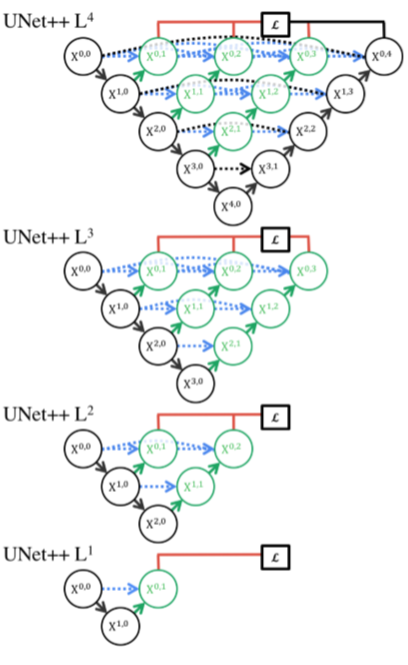
\includegraphics[scale=0.5]{figuras/unetppPrune.png}
\caption{Pruning structure of UNet++. }
\label{fig:unetppPrune}
\end{figure}

\subsection{UNet+++}
\subsubsection{Motivation}
After UNet and UNet++, we also try UNet+++\cite{unet_ppp},
which was developed and published in 2020 and maybe the latest UNet-like deep learning network.
In the following sections, we first briefly introduce UNet+++ according to the paper, and then introduce our training methods and results.

\subsubsection{Network description}
In image segmentation, Combining multi-scale features is one of important factors for accurate segmentation.
In recent deep learning network like UNet and UNet++, feature maps in different scale explore distinctive information. Lowlevel detailed feature maps capture rich spatial information, 
while high-level semantic feature maps embody position information. 
Nevertheless, these exquisite signals may be gradually diluted when progressively down- and up-sampling.
However, by implementing full-scale skip connections, UNet+++ can make full use of the multi-scale features, incorporating low-level details with high-level semantics from feature maps in different scales. 
Figure./ref{fig:unetpppGraph} shows simplified overviews of UNet+++. The image is from \cite{unet_ppp}.

\begin{figure}[!htpb]
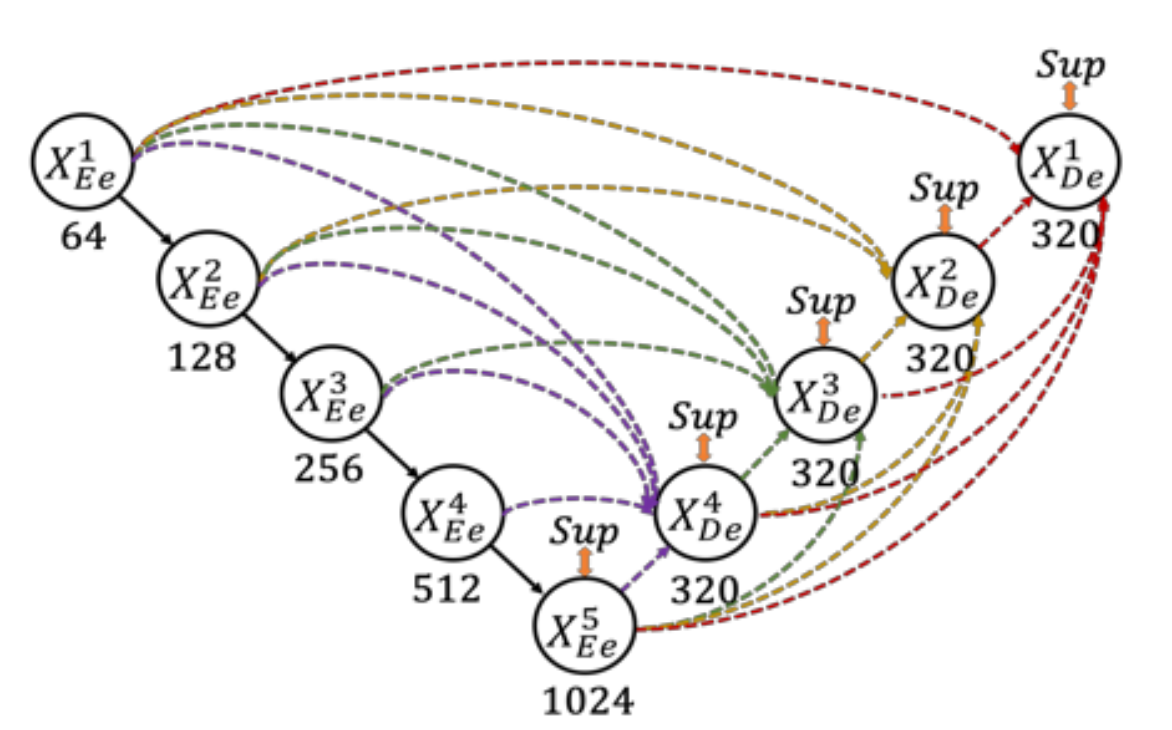
\includegraphics[width=\linewidth]{figure/unet3+.png}
\caption{UNet+++ network structure}
\label{fig:unetpppGraph}
\end{figure}
\section{Algorithm}
\subsection{U-Net}
There are mainly 3 tricks to train a U-Net, namely overlap-tile strategy, data augmentation and weighted loss.
\subsubsection{Overlap-tile strategy}
This strategy allows the seamless segmentation of arbitrarily large images. See Figure~\ref{fig:overlap}
To predict the pixels in the border region
of the image, the missing context is extrapolated by mirroring the input image.
This tiling strategy is important to apply the network to large images, since
otherwise the resolution would be limited by the GPU memory.
\begin{figure}[!htpb]
    \centering
    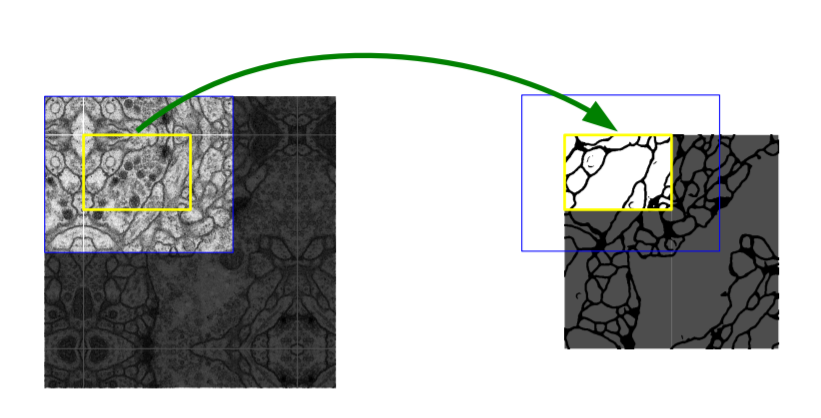
\includegraphics[scale=0.3]{figuras/overlap-tile.PNG}
    \caption{ Overlap-tile strategy for seamless segmentation of arbitrary large images. Prediction of the segmentation in
    the yellow area, requires image data within the blue area as input. Missing input data
    is extrapolated by mirroring}
    \label{fig:overlap}
    \end{figure}
\subsubsection{Data augmentation}
As for our tasks there is very little training data available, we use excessive
data augmentation by applying elastic deformations to the available training images. This allows the network to learn invariance to such deformations, without
the need to see these transformations in the annotated image corpus. This is
particularly important in biomedical segmentation, since deformation used to
be the most common variation in tissue and realistic deformations can be simulated efficiently. 

In case of microscopical images we primarily need shift and rotation invariance as well as
robustness to deformations and gray value variations. Especially random elastic deformations of the training samples seem to be the key concept to train
a segmentation network with very few annotated images. We generate smooth
deformations using random displacement vectors on a coarse 3 by 3 grid. The
displacements are sampled from a Gaussian distribution with 10 pixels standard
deviation. Per-pixel displacements are then computed using bicubic interpolation. Drop-out layers at the end of the contracting path perform further implicit
data augmentation.
\subsubsection{Weighted loss}
We pre-compute the weight map for each ground truth segmentation to compensate the different frequency of pixels from a certain class in the training
data set, and to force the network to learn the small separation borders that we
introduce between touching cells. 

The separation border is computed using morphological operations. The
weight map is then computed as
$$
w(\mathbf{x})=w_c(\mathbf{x})+w_0\cdot \exp \left(- \frac{(d_1(\mathbf{x})-d_2(\mathbf{x}))^2}{2\sigma^2}\right)
$$
where $w_c: \Omega \rightarrow R$ is the weight map to balance the class frequencies, $d_1: \Omega \rightarrow R$ denotes the distance to the border of the nearest cell and $d_2: \Omega \rightarrow R$ the distance
to the border of the second nearest cell. 
%\section{Algorithm}
\subsection{UNet++}
There are several unique algorithms and tricks used in UNet++, including deep supervision and its unique loss function. We will discuss all these below in detail.
\subsubsection{Deep supervision}
We have mentioned deep supervision in the last part about the description of UNet++, here we will discuss it in detail.\\
Let's reflect on Figure.\ref{fig:unetppStructure}, where all the outputs of the four branches connect to a single loss function. It's worth noticing that, in normal deep supervision procedure, losses at supervision layers decay with time, while in this setup, no loss would decay through time. This was because of the proposition that UNet++ was designed to support pruning during inference time, which can be done through only taking the output at layer $X^{0,t}, t\in \{1,2,3,4\}$. As a result, the deep supervision in UNet++ is not in its d=standard form, whose effects will be discussed in the experiment section.\\
\subsubsection{Loss Function of UNet++}
In the paper\cite{unet_pp}, the loss function at arbitrary output point has a uniform formula, which consists of a cross-entropy term and a Dice-coefficient term:
\begin{equation}
    \displaystyle L(Y, \hat Y)=-\frac{1}{N}\sum_{b=1}^{N}(\frac12 * Y_b * log\hat Y_b + \frac{2* Y_b*\hat Y_b}{Y_b + \hat Y_b})
\end{equation}

Where $Y_b$ and $\hat Y_b$ denote the flattened probability vector output for the $b^{th}$ image.\\

Totalling all these things together, we can see that UNet++ has 4 streams of constant gradient flow feeding back into the network during training time.

\subsection{UNet+++}
We use Pytorch to train UNet+++, so we use Pytorch's loss function and optimizer.

In details, because the result picture only have two class 0,1 per pixel, we use loss function BCEWithLogitsLoss, it combines a Sigmoid layer and the BCELoss. 
BCELoss is a criterion that measures the Binary Cross Entropy between the target and the output, the formula is:
\[\begin{aligned}
    &\mathbf{l}(\mathbf{x}, \mathbf{y})=\{l_1, \cdots, l_N\}^T, \\
    &l_n=-w_n[y_n\cdot\log{x_n}+(1-y_n)\cdot\log{(1-x_n)}]
\end{aligned}\]
Where N is the batch size. BCEWithLogitsLoss is more numerically stable than using a plain Sigmoid followed by a BCELoss as, 
by combining the operations into one layer, we take advantage of the log-sum-exp trick for numerical stability.

We use Adam algorithm as optimizer. Actually we test Adam, RMSprop, SGD and we find that Adam performs best.

\section{Experimental Settings}
\subsection{U-Net}
Here we briefly descirbe the environment and tools we use to train a U-Net ourservles. We use TensorFlow with Keras API, and the training is done on a NVIDIA GTX 1060 (6GB). We use standard Adam optimizer with learning rate 1e-4, and train the net for 10 epochs for 5 hours, each epoch containing 2000 steps. The data augmentation is done via Keras ImageGenerator API, with rotation, shift and horizontal flip.
\section{Experimental Settings}
\subsection{UNet++}
We will discuss the settings of UNet++ throughout our experiments in this section. The network structure was the same as depicted in Figure.\ref{fig:unetStructure}. Due to the limited capacity of our hardware, the training time batch size was very limited, which is actually only 1 picture per batch. We understand the effect that small batch size hinds convergence, but we had no choice. The optimizer was SGD, with a learning rate of 1e-3, momentum of 0.9 and weight decay of 1e-4. We were only able to train the network for 100 epochs due to the limited memory.


\subsection{UNet+++}
We use the given dataset to train and test the network, the learning rate is the default value(0.001) of torch.optim.Adam.
Because the network is complex, we can only set batch size to 1, otherwise the GPU memory is not enough.
\section{Result}
\subsection{U-Net}
\section{Result}
\subsection{UNet++}
We trained UNet++ with the designated parameters, along with deep supervision and without supervision, which results in the accuracies in Table.\ref{tab:unetppResult}.

\begin{table}[!htbp]
\centering
\caption{UNet++ results}\label{tab:unetppResult}
\begin{tabular}{c|c|c|c|c}
\hline
& Out 1&Out 2&Out 3&Out 4\\    
\hline
with deep supervision & 0.878 & 0.886 & 0.891 & 0.894\\
without deep supervision & / & / & / & 0.917\\
\hline
\end{tabular}
\end{table}

As shown in Table.\ref{tab:unetppResult}, deep supervised network performance increases with output layer, while still performing worse than the network without deep supervision, where in the UNet++ paper\cite{unet_pp}, the gap was not that big, and deep-supervised network perform generally better than normal ones. We suppose that was caused by our non-ideal training parameter setting. We tend to think that deep-supervised networks actually converge slower in this setting because of two reasons:
\begin{itemize}
    \item Non-decaying deep supervision force the network to figure out a good approximation right at the beginning of the network, which may over-exploit the potential of the first layer, leaving less work to do for the following layers, and making the network less competent as a whole. We argue that this setup actually slows down the training process, which will be shown in the other experiments.
    \item Small training epochs lead to early exit and non-optimal performance during training.
\end{itemize}

\subsection{UNet+++}
We test the relationship between epoch and the accuracy of test data, in order to find the best epoch value. In the test, the value of epoch range from 1 to 40. 
In each iteration, we test the current model on test dataset, and record the accuracy. The result is given in the following image.

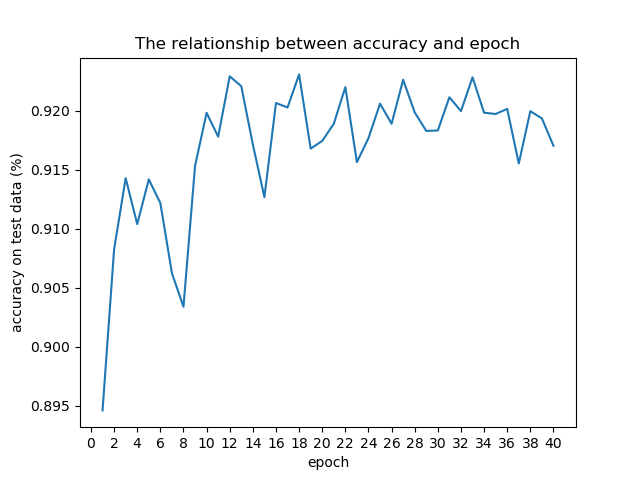
\includegraphics[width=\linewidth]{figuras/epoch_accuracy.png}

The image shows that as the epoch value increase, the accuracy first increase rapidly and than decrease slowly, 
which means that when epoch is too large, it becomes overfitting.
The best accuracy is 0.923, with the epoch value 18

%\section{Conclusão}
A seção de conclusões não é obrigatória. Embora esta possa rever os pontos principais do artigo, não duplique o resumo como conclusão. A conclusão deve discorrer sobre a importância do trabalho ou sugerir aplicações e extensões.

%Exemplo de comentario
\begin{comment}
Aqui também é um comentário
\end{comment}
\section{Conclusion}
In the project, we study the deep learning network UNet, UNet++ and UNet+++, and implement all three network on the given dataset.
The experiments on the three network show lots of information. First, all experiments get relatively high accuracy on test data, which means that UNet and its variants work well in image segmentation.
Second, these network can converge quickly. In the training process, Although the given training dataset is not big(25 images), the accuracy reaches highest when iterate for about 20 times, a relatively small value.
Third, the modification for Unet in other two networks improve the network performance, especially UNet+++. The best accuracy of UNet and UNet++ is approximately 0.918, and that of UNet+++ can be 0.923, a impovement of 0.5\%.

In conclusion, we learn a lot from the project. We get a better understand of image segmentation and deep learning. 
However, Because of time limit and device limit, our experiments lack further optimization on some parameter, so the accuracy in some experiments above can be higher. We may refine it in the futrue.



\printbibliography

\section*{Autores}

\begin{wrapfigure}{l}{0.3\linewidth}
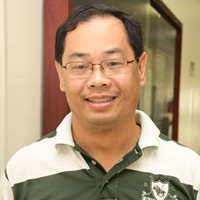
\includegraphics[width=\linewidth]{figuras/autor1.jpg}
\end{wrapfigure}

 \textbf{Carlos Alberto Ynoguti} Possui graduação em Engenharia Elétrica pela Universidade de São Paulo(1991), mestrado em Engenharia Elétrica pela Universidade de São Paulo(1995), doutorado em Engenharia Elétrica pela Universidade Estadual de Campinas(2000) e pós-doutorado pela Universidade Estadual de Campinas(2001). Atualmente é Professor Adjunto do Instituto Nacional de Telecomunicações e Membro de corpo editorial da Telecomunicações (Santa Rita do Sapucaí) (1516-2338). Tem experiência na área de Engenharia Elétrica, com ênfase em Telecomunicações. Atuando principalmente nos seguintes temas:processamento digital de sinais, processamento de voz, reconhecimento de fala. 

\begin{wrapfigure}{l}{0.3\linewidth}
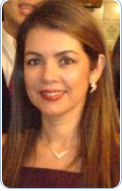
\includegraphics[width=\linewidth]{figuras/autor2.png}  
\end{wrapfigure}

   \textbf{Rosanna Mara Rocha Silveira} Possui graduação (1985) em Ciência da Computação pela UFMG (Universidade Federal de Minas Gerais) e mestrado (2003) em Engenharia Elétrica pela UNICAMP (Universidade Estadual de Campinas). Atualmente é professora adjunta da Fundação Instituto Nacional de Telecomunicações (INATEL). Na área de Engenharia tem atuação nas seguintes subáreas: algoritmos, estruturas de dados, banco de dados, modelagem e simulação, simulação de evento discreto, métodos numéricos, redes de comunicação sem fio, múltiplo acesso, análise e desempenho de redes de comunicação, processamento de sinais, transformadas wavelets e compressão de sinais.

\begin{wrapfigure}{l}{0.3\linewidth}
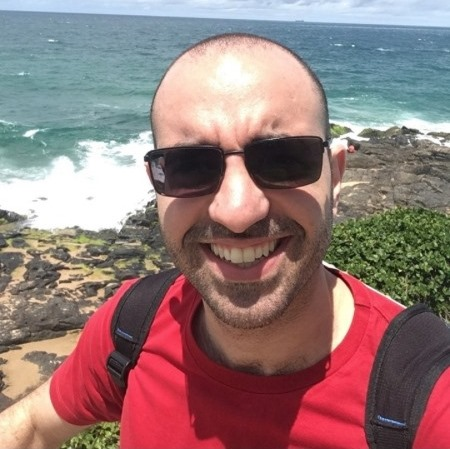
\includegraphics[width=\linewidth]{figuras/autor3.png}
\end{wrapfigure}

    \textbf{Phyllipe Lima} é Doutorando em Computação Aplicada pelo INPE - Instituto Nacional de Pesquisas Espaciais, na área de Engenharia de Software realizando estudos sobre metadados através da análise estática de código fonte e MSR (Mining Software Repositories). Mestre em Ciência da Computação(2016) pela UNIFEI - Universidade Federal de Itajubá. Engenheiro de Telecomunicações(2011) pelo INATEL - Instituto Nacional de Telecomunicações.  Técnico em Telecomunicações(2006) pela Escola Técnica de Eletrônica - ETE "FMC". É professor auxiliar do INATEL, atuando nos cursos de Engenharia da Computação e Engenharia de Software. Tem interesse nas áreas de Engenharia de Software Empírica, Desenvolvimento de Jogos e Computação Gráfica.


   
   
   
   
   

\end{document}
